\documentclass[10pt,conference]{IEEEtran}
\IEEEoverridecommandlockouts
% The preceding line is only needed to identify funding in the first footnote. If that is unneeded, please comment it out.
%Template version as of 6/27/2024

\usepackage{cite}
\usepackage{amsmath,amssymb,amsfonts}
\usepackage{algorithmic}
\usepackage{graphicx}
\usepackage{textcomp}
\usepackage{xcolor}
\def\BibTeX{{\rm B\kern-.05em{\sc i\kern-.025em b}\kern-.08em
    T\kern-.1667em\lower.7ex\hbox{E}\kern-.125emX}}
\begin{document}
\title{Parametric Benchmark Generation for Domain-Agnostic Relational Document Understanding}

% NOTE: CASCON review is DOUBLE-BLIND -- this author block must be
% removed (or anonymized) before submitting the PDF to EasyChair.
\author{\IEEEauthorblockN{1\textsuperscript{st} Farees Siddiqui}
\IEEEauthorblockA{\textit{Faculty of Science} \\
\textit{Ontario Tech University}\\
Oshawa, Canada \\
farees.siddiqui@ontariotechu.net}
\and
\IEEEauthorblockN{2\textsuperscript{nd} Dr. Ken Pu}
\IEEEauthorblockA{\textit{Faculty of Science} \\
\textit{Ontario Tech University}\\
Oshawa, Canada \\
ken.pu@ontariotechu.net}
}


\maketitle

\begin{abstract}
Abstract goes here. Do not use symbols, special characters, footnotes, or math
in the title or abstract. CASCON also asks separately for a 200--250 word
poster abstract for the website upon acceptance.
\end{abstract}

\begin{IEEEkeywords}
keyword, keyword, keyword
\end{IEEEkeywords}

\section{Introduction}

\section{Approach}

\section{Preliminary Results}

\begin{table}[htbp]
\caption{Table caption.}
\begin{center}
\begin{tabular}{|c|c|c|}
\hline
\textbf{Head} & \textbf{Head} & \textbf{Head} \\
\hline
 &  &  \\
\hline
\end{tabular}
\label{tab1}
\end{center}
\end{table}

\begin{figure}[htbp]
\centerline{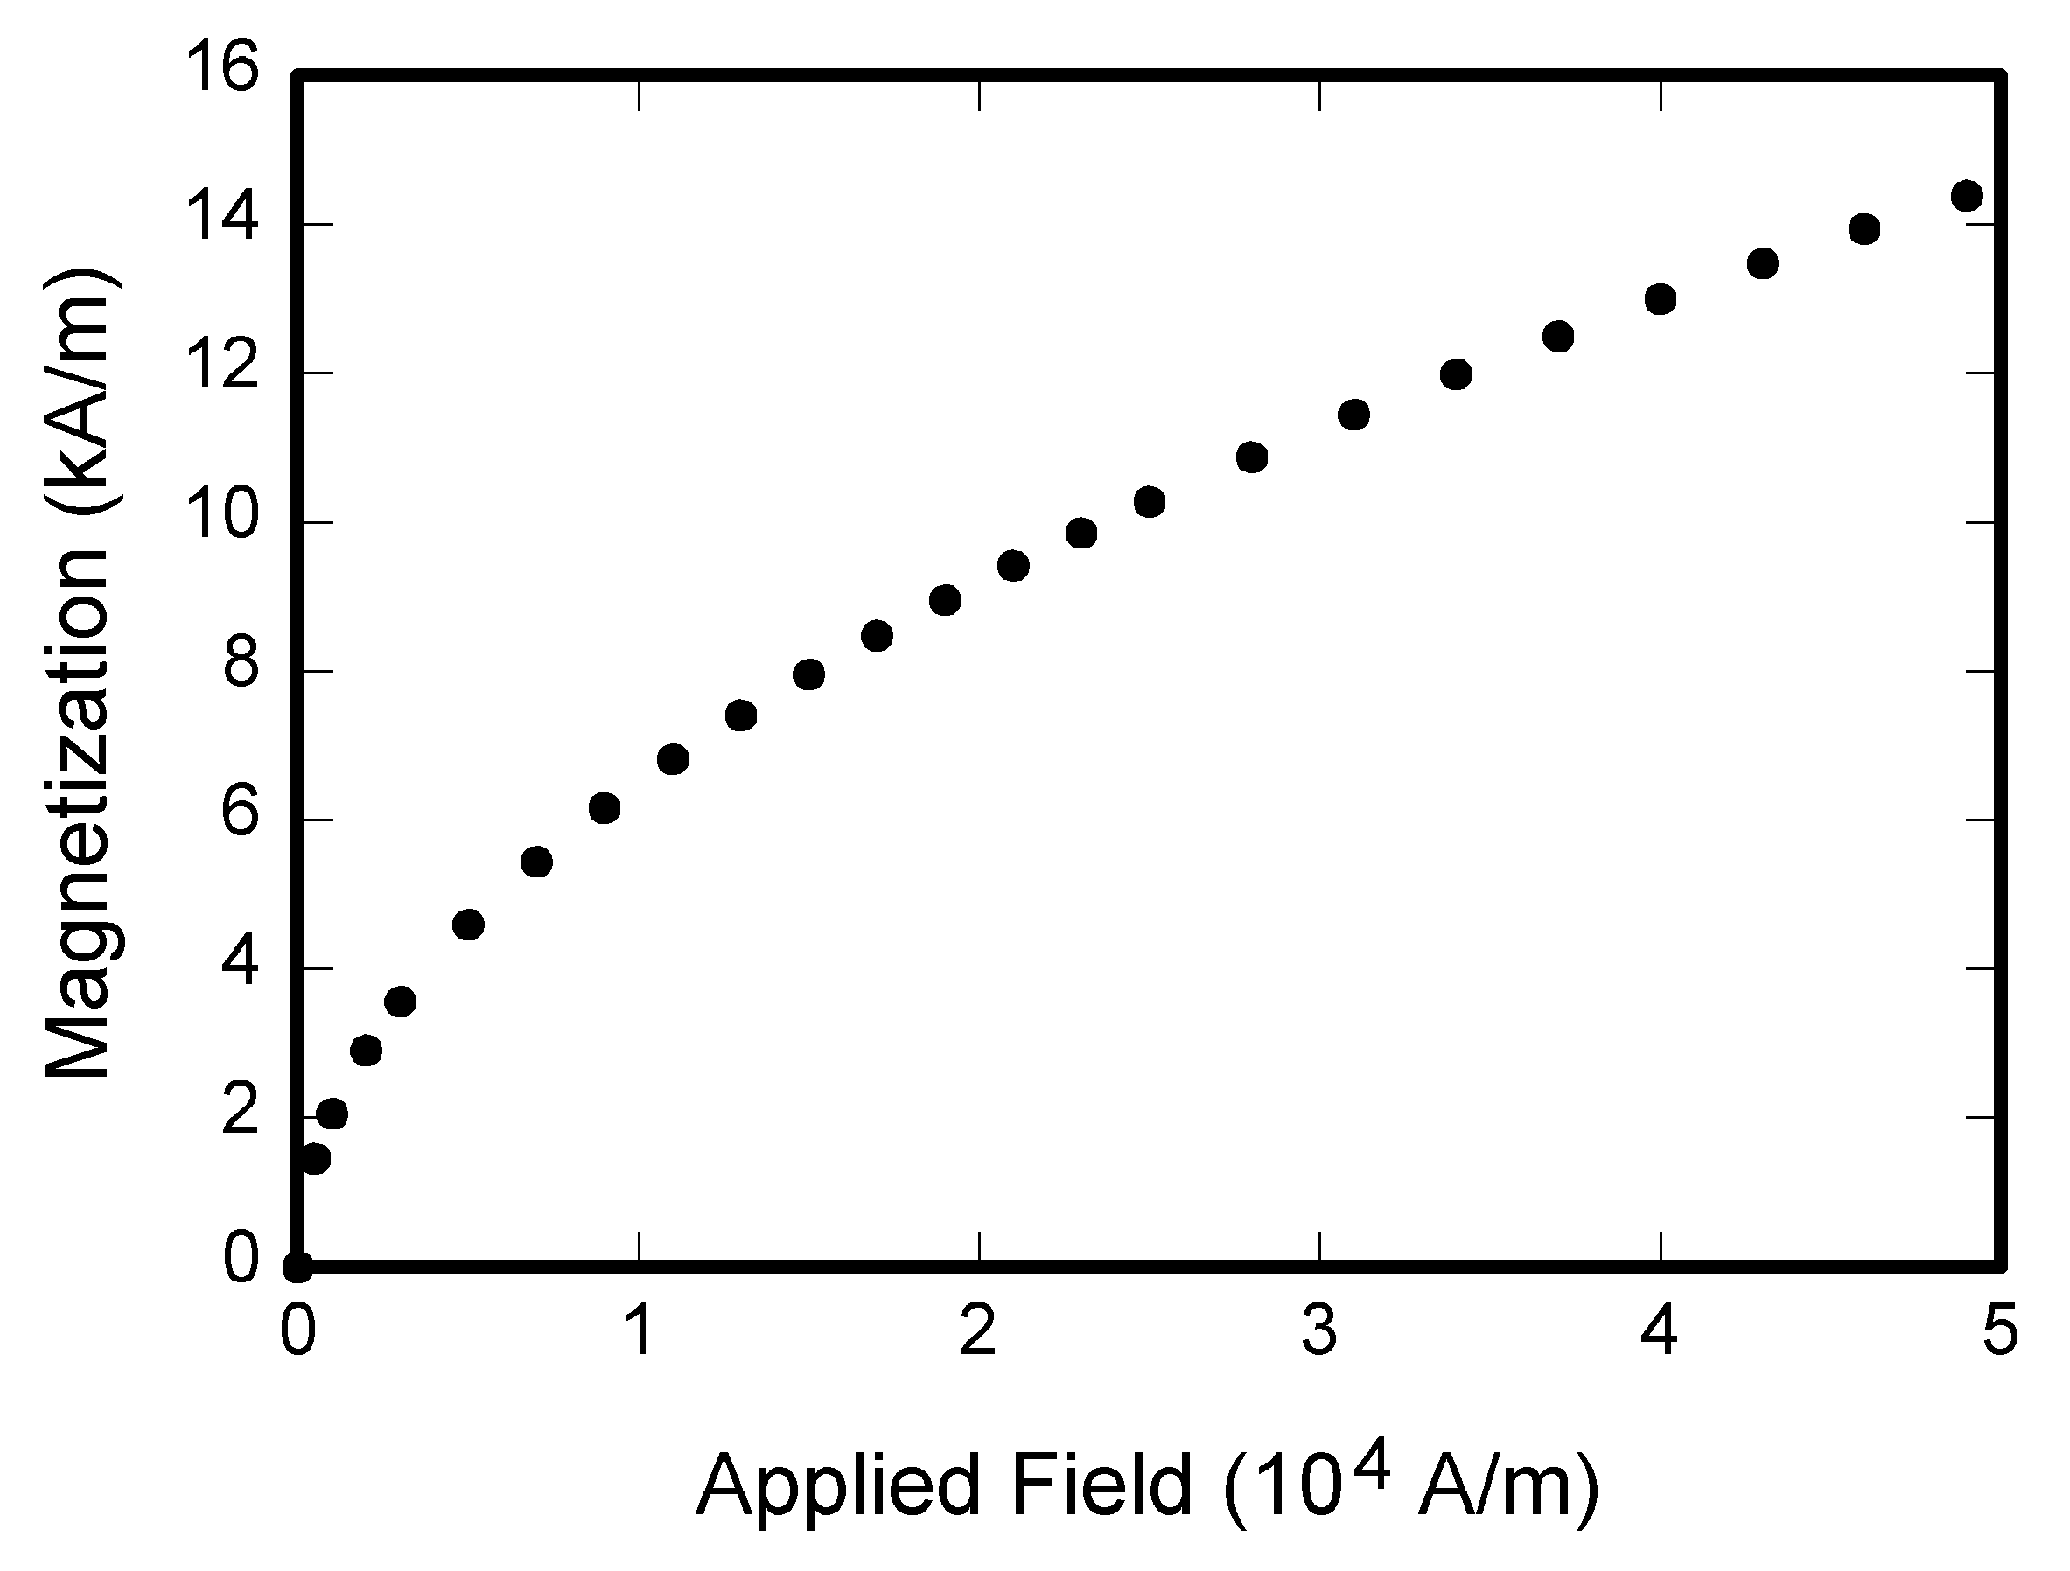
\includegraphics{fig1.png}}
\caption{Figure caption.}
\label{fig}
\end{figure}

\section{Conclusion}

\begin{thebibliography}{00}
\bibitem{b1} A. Author, ``Title of paper,'' in \emph{Proc. Conf.}, 2025, pp. 1--10.
\end{thebibliography}

\end{document}
